%=========================================================================
% (c) Michal Bidlo, Bohuslav Křena, 2008

\chapter{Úvod}

\chapter{Teoretický rozbor}
\section{Síťové modely}

Síťový model je poměrně složitý a z toho důvodu se pro jeho popis i implementaci využívají na sobě nezávislé vrstvy, kde každá vrstva pracuje s vlastním datovými strkturami a vůbec netuší co se děje na ostatních vrstva.
Tyto datové struktury se nazývají XXX


\subsection{ISO/OSI}
ISO/OSI model je používán pouze jako referenční model, není známo jeho reálné použití v počítačových sítích.
Tento model je rozdělen na 7 vrstev.

\begin{itemize}
\item{Fyzická vrstva / Vrstva síťového rozhraní}
\item{Linková vrstva}
\item{Síťová vrstva}
\item{Transportní vrstva}
\item{Relační vrstva}
\item{Prezentační vrstva}
\item{Aplikační vrstva}
\end{itemize}

\begin{figure}[!htb]
\centering
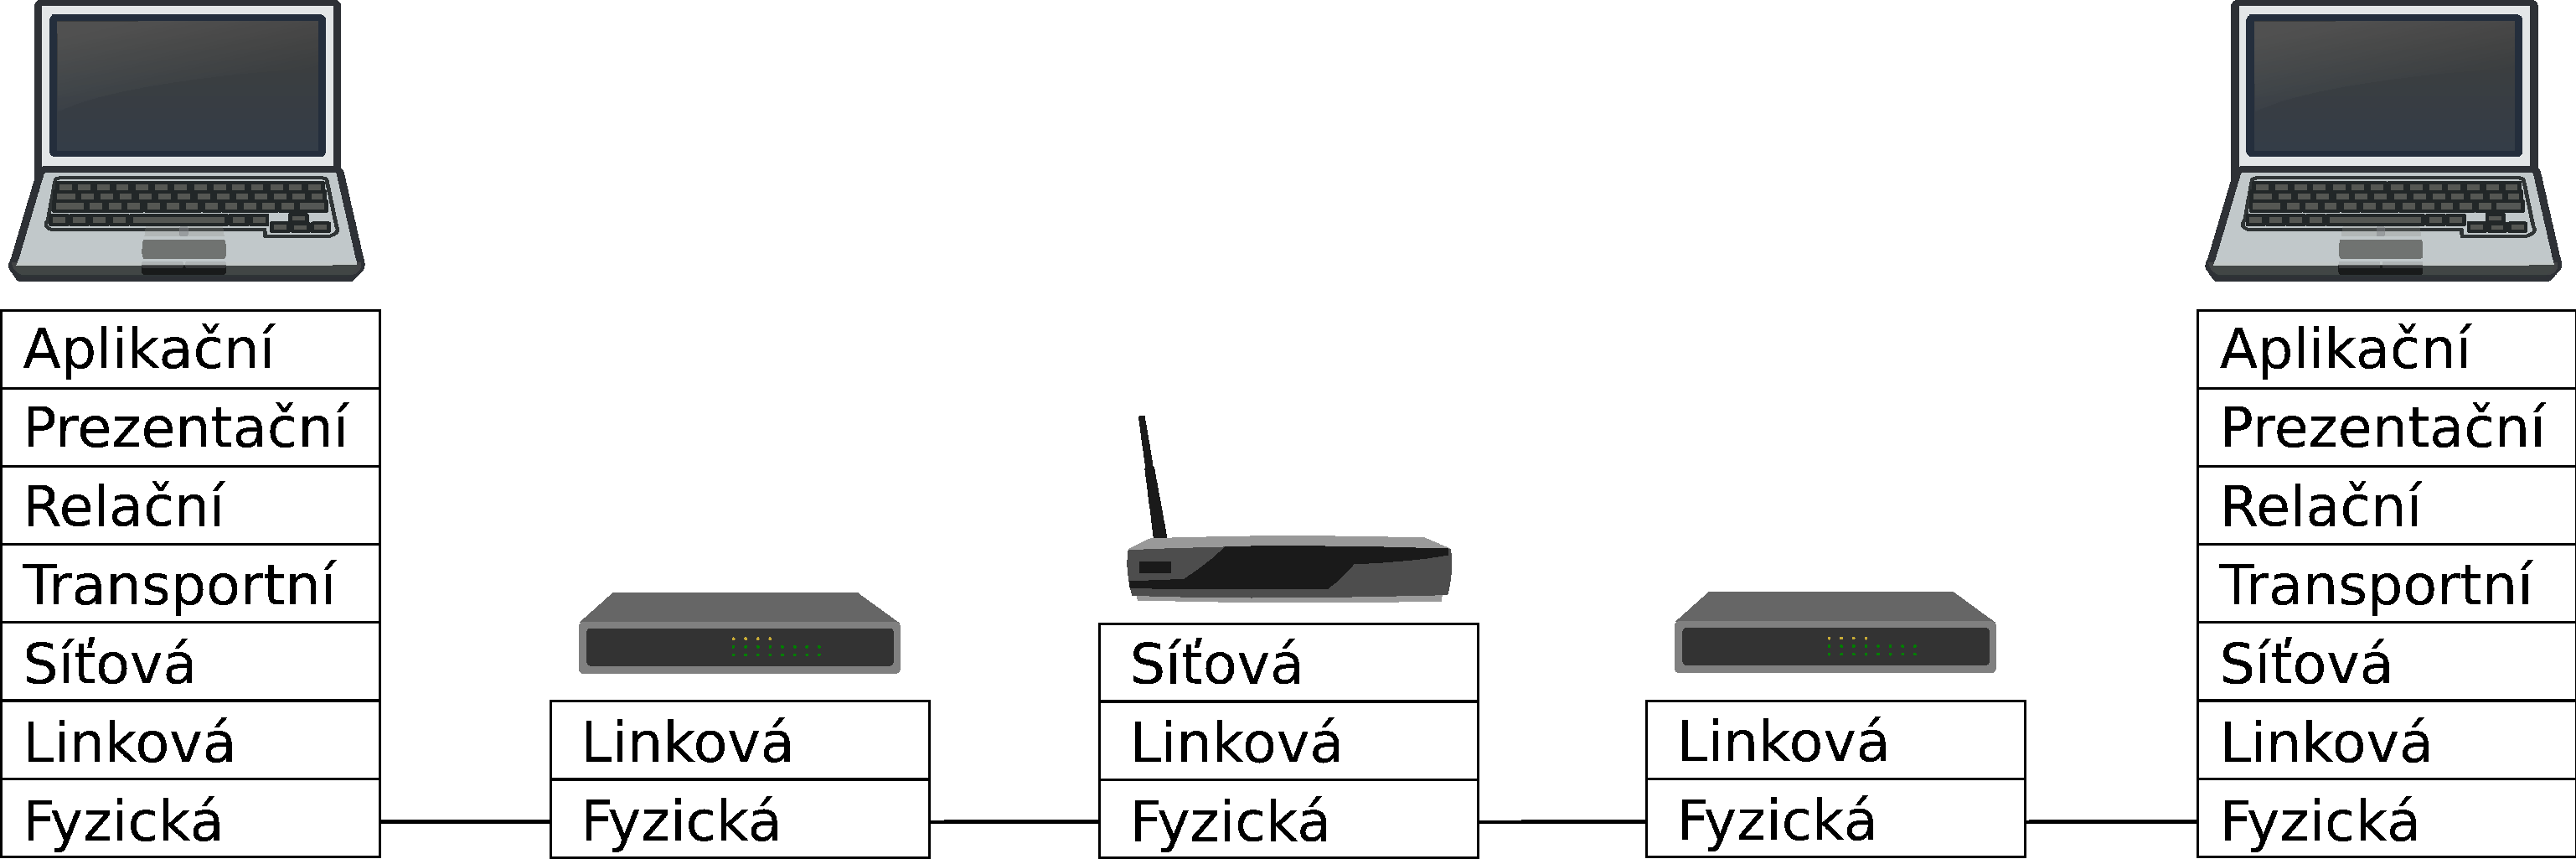
\includegraphics[scale=.25]{fig/layers.pdf}
\caption{Znázornění průchodu dat počítačovou sítí}
\label{fig:layers}
\end{figure}

\subsubsection{Fyzická vrstva / Vrstva síťového rozhraní}
Nejnižší vrstva v obou zmíněných modelech pracuje s daty na úrovni bytů a stará se o jejich přenos po přenosovém médiu.

\subsubsection{Linková vrstva}
Linková vrstva pracuje s datovou strukturou nazývanou rámec.
Rámec obsahuje informace o fyzických adresách obou účastníků komunikace.
Dále se stará o detekci chyb při přenosu na nižší vrstvě, fyzické.
Technologie se kterou se je možné nejvíce setkat se Ethernet.
Na této vrstvě pracují zařízení jako je switch, hub.

\subsubsection{Síťová vrstva}
Na této vrstvě probíhá komunikace za využití IP adres. Prvky používané na této vrstvě jsou nazývaný routery.
Účelem těcho zařízení je směrování paketů procházejících sítí. K tomu využívají směrovací tabulku na optimalizace jejího prohledávání
se věnuje část této práce zabývající se problémem vyhledávání nejdelšího shodného prefixu.
Datové struktury jsou pojmenované pakety.
Pakety obsahují

\subsubsection{Transportní vrstva}
Transportní vrstva pracuje s datovou strukturou zvanou segmenty. Obsahují informace jako je kontrolní součet pro zjištění integrity dat,
pořadové číslo rámce pro spojení dat, která byla na cestě k cíli rozdělena na více částí a také obsahuje čísla portů
pro určení uživatelských aplikací, která data odeslala a která je na druhém konci má přijmout.

Transportní vrsta (a všechny vyšší) se tradičně již nevyskytuje na síťových zařízeních, která se starají o provoz.
Slouží až pro koncové stanice aby mohli určit program, kterému budou data předána.

\subsubsection{Relační vrstva}


\subsubsection{Prezentační vrstva}


\subsubsection{Aplikační vrstva}
Aplikační vrstva je vrstva, kde pracují uživatelské aplikace.
Na této vrstvě může docházet ke kontrole přenášeného obsahu a k detekci možný útoků na uživatelské aplikace.

\subsection{IP}
Model IP je narozdíl od ISO/OSI modelu nejpoužívanějším síťovým modelem ve světě.
Skládá se pouze ze čtyř vrstev a ty jsou:

\begin{itemize}
\item{Vrstva síťové rozhraní}
\item{Síťová vrstva}
\item{Transportní vrstva}
\item{Aplikační vrstva}
\end{itemize}

\section{Časově kritické operace}
S neustálím zvyšováním požadavků na rychlost síťového připojení také rostou nároky na rychlost
algoritmů, které na síťových zařízeních pracují. Při rychlostech, které jsou dnes reálné je problém se zpracováním
síťových operací, které mají k dispozici pouze několik desítek procesorových instrukcí pro zpracování jednoho požadavku
pokud bereme v úvahu veřejností používané procesory.

Proto v posledních letech nabírá na obrátkách trend pro využítí ASIC čipů nebo programovatelných hradlových polí.
Tyto prvky totiž umožňují rychlejší zpracování s řádově menšími požadavky.
Tohoto rychlostního rozdílu je dosaženo právě díky specializaci čípů na provádění jedné specializované operace na což jsou uzpůsobeny
narozdíl od obecných procesorů, které musejí zvládat mnohem větší repertoár operací.

\subsection{Hledání nejdelšího prefixu}
Hledání nejdelšího shodného prefixu se používá při směrování paketů.
Pro docílení nejlepší efektivity při přeposílání paketů je nutné znát co nejpřesněji další místo, na které je paket třeba doručit.
Toho je řešeno prohledáváním routovací tabulky.
Pro dosažení větší rychlosti je routovací tabulka v paměti směrovače uložena v jiných strukturách, které tabulce neodpovídají.
V této práci jsou pro uložení routovací tabulky využity algoritmy {\tt Binary search on prefix length} a {\tt TreeBitmap}.
Oba jsou variací obecně n-árního stromu.

\subsection{Hledání podřetězců}
Pro hledání potřetězců je implementován algoritmus autorů Aho a Corasicové. Tento algoritmus používá pro zjištění shody s podřetězcem konceptu konečného automatu. Při každé iteraci algoritmu se provede přechod o jeden znak.

\subsubsection{Aho-Corasick}
efektivita aho-coracick algoritmu je velkým dílem závislá na tom, zda se veškerá paměť použitá k uložení vyhledávaných slov veljde do cache paměti stroje, na kterém poběží.

Na klasickém desktopovém počítači je několik vrstev cache pamětí.
Pokud budeme brát v úvahu jednotlivé vrstvy samostatně, tak do
velikost jednoho stavu automatu se může výrazně lišit v závislosti počtu následovníků a počtu
pravidel, které nejsou přímo v tomto stavu, ale jsou to podřetězce tohoto stavu.
Tyto podřetězce byly zjištěny iterativním procházením automatu od hloubky 0 a procházení tzv. failure cest, kdy každý stav navštívený failure průchodem obsahující pravidlo znamená že stav, pro který se hledá failure cesta obsahuje podpravidlo vyhovující právě tomuto stavu.
L1 se vejde XXXXX stavů automatu, což může reprezentovat právě XXX slov o délce NNNN znaků.
L2 se vejde XXXXX stavů automatu, což může reprezentovat právě XXX slov o délce NNNN znaků.
L3 se vejde XXXXX stavů automatu, což může reprezentovat právě XXX slov o délce NNNN znaků.
L4 se vejde XXXXX stavů automatu, což může reprezentovat právě XXX slov o délce NNNN znaků.

\subsubsection{Regulární výrazy}

TODO konstrukce NFA
TODO konstrukce DFA z NFA
TODO konstrukce MDFA z DFA
== 3 strany


\subsection{}

\chapter{Návrh API knihovny}
Knihovna je navržena s důrazem na snadnou rozšiřitelnost případnými dalšími algoritmy.
Knihovna je taktéž navržena tak, aby bylo velmi snadné používat pouze jednu z operací, které knihovna implementuje.
To je vhodné pro použití v úzce specializovaných zařízení, jimž tak bude stačit menší množství paměti pro uložení knihovny.
Každá podknihovna lze vytvořit jedním příkazem ve své složce a také poskytuje vlastní rozhraní, které lze vložit do používaných algoritmů.

hlavičkové soubory jsou rozděleny na veřejné a privátní rozhraní, kde privátní rozhraní je používáno pouze uvnitř knihovny. Hierarchickou strukturu je možné vidět na obrázku \ref{fig:header-dependecies}.

Jako výchozí hlavičkový soubor je použit types.h, který obsahuje definice datových struktur pro všechny algoritmy v podknihovně, které musí být viditelné i z veřejného rozhraní. Dalším souborem je types-precompiled.h, který je generován z types.h při překladu když se vybírá používaný algoritmus. common.h je hlavičkový soubor společný pro všechny algoritmy v podknihovně a algortihm.h pak obsahuje deklarace právě pro jeden konkrétní algoritmus.
sublib.h je pak hlavičkový soubor, který tvoří veřejné rozhraní ke knihovním funkcím.

\begin{figure}[!htb]
\centering
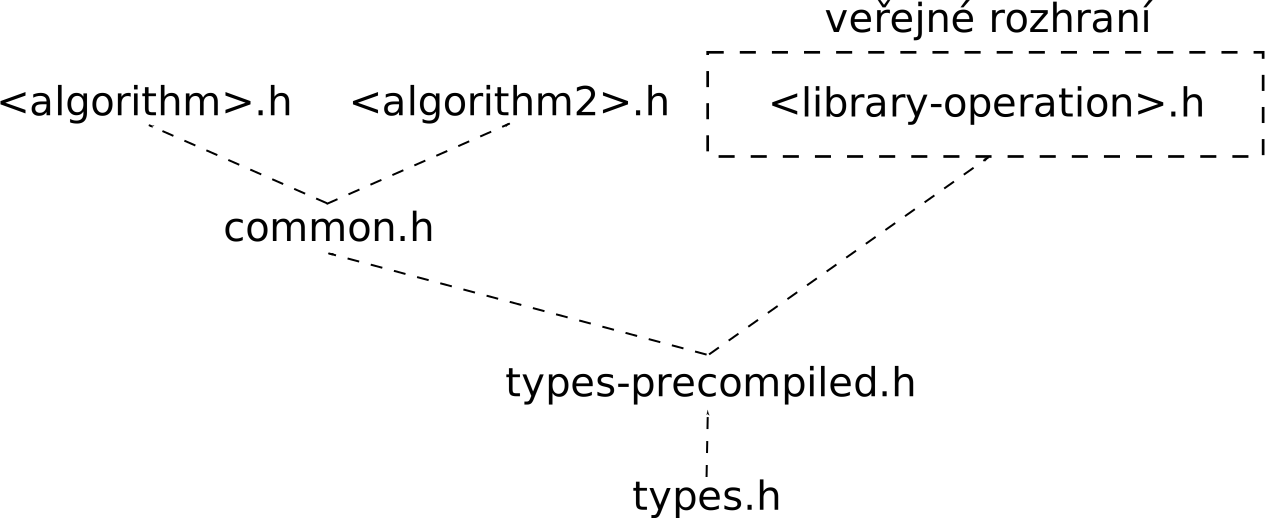
\includegraphics[scale=.25]{fig/header-dependencies.pdf}
\caption{Diagram závislostí hlavičkových souborů}
\label{fig:header-dependecies}
\end{figure}

Důvod pro vlastní implementaci regulární výrazů je možnost zvolit nejvhodnější algoritmus pro danou operaci.
Dalším důvodem je převod implementace do akcelerovaného hardware.
Nějvýznamějším důvod pro vlastní implementaci je provádění několika regulárních výrazů najednou na jednom vstupní textu a vracení čísla regulárního výrazu, který vstupnímu textu vyhovuje, což není možné docílit při použití stadardní implementace ze stdlib, {\tt regex}

\chapter{Výsledky}
\section{Hledání nejdelšího shodného prefixu}

\chapter{Závěr}
Závěrečná kapitola obsahuje zhodnocení dosažených výsledků se zvlášť vyznačeným vlastním přínosem studenta. Povinně se zde objeví i zhodnocení z pohledu dalšího vývoje projektu, student uvede náměty vycházející ze zkušeností s řešeným projektem a uvede rovněž návaznosti na právě dokončené projekty.

\section{Další vývoj projektu}

Jako další kroky pro vylepšení knihovny bych zvolil optimalizaci implementovaných algoritmů dle

%=========================================================================
